\documentclass[journal,a4paper]{IEEEtran}
\usepackage{cite}
\usepackage{amsmath,amssymb}
\usepackage{graphicx}
\usepackage{booktabs}
\usepackage{multirow}
\usepackage{url}
\usepackage[hidelinks]{hyperref}
\graphicspath{{figures/}}

\begin{document}

\title{Component Scores Do Not Compose: A Held-Out Study of\\
Clause Detection, Span Extraction and Risk Prioritization on CUAD}

\author{Jerin~Aktar,~Afnan~Mazumdar,~and~Shoyeb~Hasan~Sayem
\thanks{The authors are with the Department of Computer Science and Engineering,
BRAC University, Dhaka 1212, Bangladesh (e-mail: afnan.mazumdar@g.bracu.ac.bd).}
\thanks{Supervised by Utsha Kumar Roy, Department of CSE, BRAC University.}}

\markboth{BRAC University, Department of Computer Science and Engineering}%
{Aktar \MakeLowercase{\textit{et al.}}: Component Scores Do Not Compose}

\maketitle

\begin{abstract}
Automated contract review is usually evaluated one component at a time. We report a
three-stage pipeline on the Contract Understanding Atticus Dataset (CUAD) --- clause
presence, span extraction, and a category-level risk layer --- evaluated on a strict
contract-level 80/20 split, and show that its component scores substantially overstate
what the assembled system delivers. A sliding-window DistilBERT trained under multiple-instance
learning \emph{loses} to a full-document TF--IDF baseline (micro-F1 0.694 against 0.775).
We eliminate four alternative explanations: training on all 53{,}662 window examples rather
than a 24{,}000 subsample moves micro-F1 by $-0.0004$; three random seeds put the gap at 9.5
standard deviations; six aggregation rules at their own optimal thresholds all remain behind
the baseline; and an untuned decision threshold accounts for 0.056 of the difference. A
conjunctive ensemble reaches 0.776, but its $+0.0014$ margin is smaller than the bootstrap
interval, the seed variance and the dataset-split variance alike. Run end to end, only
21.7\% (95\% CI $[19.6, 23.9]$) of gold clauses survive all three stages against the
$\approx$64\% the component scores predict, and we localize the loss to window selection
(31.7\%) and a train/inference distribution mismatch. Finally, aggregate micro-F1 and the
system's stated purpose diverge: the configuration ranked first misses 37.5\% of high-risk
clauses while a configuration ranked last misses 13.6\%. We argue that pipeline-level and
risk-weighted evaluation should be reported alongside component metrics as a matter of course.
\end{abstract}

\begin{IEEEkeywords}
Legal natural language processing, contract analysis, CUAD, multiple-instance learning,
model evaluation, calibration, risk assessment.
\end{IEEEkeywords}

\section{Introduction}
\IEEEPARstart{C}{ommercial} contracts routinely run to tens of thousands of characters, while the
provisions that determine a signer's exposure occupy a few hundred. In CUAD~\cite{cuad}, the
median contract is 33{,}143 characters and the median annotated clause is 196 --- roughly
$16\times$ a standard transformer encoder's input window against a target two orders of
magnitude smaller. CUAD frames the resulting problem as extraction: given a category, locate
the clause. It stops there, offering no indication of what a located clause means for the party
signing it.

This paper reports a system that attempts the further step and, more usefully, an evaluation of
where that system fails. Our contributions are:

\begin{enumerate}
\item A negative result on long-document presence classification, with four alternative
explanations tested and eliminated (Section~\ref{sec:controls}).
\item A demonstration that stage-wise scores do not compose: 21.7\% end-to-end survival against
$\approx$64\% predicted, decomposed into two identifiable causes (Section~\ref{sec:e2e}).
\item Evidence that aggregate micro-F1 and user harm can invert the model ranking, measured
through a risk-weighted evaluation (Section~\ref{sec:risk}).
\item A demonstration that a small reference set can convert a generation task into
classification without the metric registering it (Section~\ref{sec:summ}).
\end{enumerate}

\section{Related Work}
CUAD~\cite{cuad} supplies 510 commercial contracts with expert annotations over 41 clause
categories, posed in SQuAD format~\cite{squad}. Domain-adapted encoders~\cite{legalbert} and
benchmark suites~\cite{lexglue} have advanced legal language understanding, but operationalize
importance as category membership rather than as severity for a particular party. We are not
aware of an established risk-severity model covering CUAD's categories, which is why the layer
we add is presented as a prototype for expert validation rather than as a validated instrument.

Long inputs are handled by retrieval, by windowing with aggregation, or by sparse
attention~\cite{longformer}. Windowed aggregation with a maximum is the classical
multiple-instance learning (MIL) rule~\cite{mil}. For generation, T5~\cite{t5} and its
instruction-tuned variant~\cite{flan} make clause simplification natural to express;
Manor and Li~\cite{manor} assemble plain-English contract summaries and observe a tendency
toward generic output. A substantial literature establishes that fluent abstractive output is
frequently unfaithful~\cite{maynez,factcc} and that overlap metrics such as
ROUGE~\cite{rouge} correlate poorly with faithfulness; embedding metrics~\cite{bertscore}
improve similarity estimation without testing factuality. Our summarization result is an
extreme case of the same phenomenon, and our calibration analysis follows~\cite{calibration}.

Two properties of CUAD dominate any modelling effort on it. The first is class imbalance: per-category
positive rates span 100\% to 2.5\%, and the median category appears in roughly 23\% of contracts.
The second is length. Because contracts exceed encoder windows by more than an order of magnitude,
every system must commit to a length strategy before it can commit to a model, and that choice is
usually asserted rather than measured. Part of our contribution is to measure it: we report a
retrieval ceiling before training and a cost benchmark for sparse attention on the target hardware,
rather than arguing either point.

Evaluation practice in this area typically reports one score per component. Where pipelines are
assembled, the assembled system is rarely scored end to end, so the compounding of stage errors goes
unquantified --- which is the gap Section~\ref{sec:e2e} addresses.

\section{Dataset and Protocol}
All experiments use CUAD v1. We split \textbf{at the contract level}, 80/20, with a fixed seed:
408 training and 102 test contracts, 20{,}910 (contract, category) rows at a 32.1\% positive
rate. The same split is loaded from disk by every model, so ``test'' denotes the same 102 unseen
contracts throughout. Positive rates per category range from 100\% (\emph{Document Name}) to
2.5\% (\emph{Source Code Escrow}); five categories have at most seven positive test contracts.

\textbf{No hyperparameter was tuned.} Learning rates, batch sizes and epochs are published
defaults; the window geometry follows from a measurement on training data; the decision
threshold is the softmax default. This protects the held-out evaluation, but means the
transformer competes at conventional settings against a baseline with essentially nothing to
tune --- a limitation we return to in Section~\ref{sec:threats}.

\section{Method}
\textbf{Presence.} A TF--IDF baseline over the entire document feeds per-category logistic
regression. In parallel, 2{,}000-character windows at a 1{,}500-character stride tile each
contract; a DistilBERT~\cite{distilbert} scores (category question, window) pairs, and the
document-level score is the maximum over windows --- the MIL rule. The 500-character overlap
exceeds the median clause length, so no clause falls between windows. Parameter-free AND, OR and
AVG rules combine the two models; nothing in them can be fitted to the test set.

Before training we measured the ceiling that a retrieval design would impose: the best query
strategy places the gold clause in its selected windows only 64.0\% of the time, below what the
baseline already achieves. Retrieval was therefore rejected on a measurement rather than an
assumption. We note the scope: this bounds \emph{lexical} retrieval only.

\textbf{Span.} A DistilBERT question-answering head predicts start and end positions. At
training time each example is re-centred so the answer begins $\approx$150 characters into a
1{,}200-character window; this uses a label to build a training example, never an inference
input.

\textbf{Risk and explanation.} Each category carries a fixed High/Medium/Low level scored from
the weaker party's perspective (8/22/11) using five criteria: financial exposure,
irreversibility, restriction of future freedom, asymmetry, and survival. This is
\emph{category-level prioritization}, not clause-level assessment. A FLAN-T5-small is fine-tuned
to map a clause to a plain-English sentence, seeded with 41 author-written category templates.

\section{Results}

\subsection{Presence Classification}
Table~\ref{tab:presence} reports micro-F1 over the 4{,}182 test decisions. The windowed
transformer loses to the lexical baseline by 0.081. A cluster bootstrap over contracts
(10{,}000 resamples; the 41 decisions within a contract are not independent) puts that gap at
$[+0.063,+0.099]$, significant in every resample. The AND ensemble finishes nominally first at
0.776, with a margin of $+0.0014$ and an interval of $[-0.0068,+0.0089]$ --- a tie.

\begin{table}[!t]
\caption{Presence models, held-out micro-F1}
\label{tab:presence}
\centering
\begin{tabular}{lccc}
\toprule
\textbf{Model} & \textbf{micro-F1} & \textbf{Prec.} & \textbf{Rec.}\\
\midrule
AND ensemble          & \textbf{0.776} & 0.772 & 0.780\\
TF--IDF baseline      & 0.775 & 0.742 & 0.810\\
Ensemble AVG          & 0.718 & --- & ---\\
Ensemble OR           & 0.696 & --- & ---\\
Transformer (max-pool)& 0.694 & 0.562 & 0.908\\
\bottomrule
\end{tabular}
\end{table}

\subsection{Four Controls}
\label{sec:controls}
A bootstrap answers whether a gap could be sampling noise; it cannot answer whether the model
was handicapped. Table~\ref{tab:controls} reports four controls.

\begin{table}[!t]
\caption{Alternative explanations for the transformer's deficit}
\label{tab:controls}
\centering
\small
\setlength{\tabcolsep}{4pt}
\begin{tabular}{lcc}
\toprule
\textbf{Control} & \textbf{Effect on micro-F1} & \textbf{Verdict}\\
\midrule
All 53{,}662 windows      & $-0.0004$ $[-0.010,+0.010]$ & none\\
Random seed, 3 runs       & SD $0.0085$; gap $9.5$ SD   & none\\
Aggregation, 6 rules      & best $0.750 < 0.775$        & none\\
Threshold, swept          & $+0.056$ at $t{=}0.90$      & partial\\
\bottomrule
\end{tabular}
\end{table}

Doubling the training data changed micro-F1 by $-0.0004$ while raising recall (0.908 to 0.927)
and lowering precision (0.562 to 0.555): more data made the model fire more readily, not more
accurately, which is what a maximum over $\approx$35 windows predicts. Reseeding moves the
ensemble by more than the margin claimed for it (SD 0.0022, range 0.0042 against $+0.0014$).
Refitting the baseline on 20 independent splits gives SD 0.0063 --- the largest of the three
uncertainties, and $4.5\times$ the ensemble margin.

An ablation over aggregation rules on identical window scores found that top-3 mean outperforms
the maximum at the default threshold (0.7144 vs 0.6943), while the maximum is best once each
rule receives its own threshold (0.7504). No rule at any threshold reaches the baseline. The
threshold control is the one that qualifies our finding: the un-chosen 0.5 boundary costs the
transformer 0.056, so part of its deficit is an operating-point artefact. We do not adopt the
swept threshold, since selecting it on test data would invalidate the held-out evaluation.

\subsection{Aggregation Ablation}
Max-pooling was adopted because it implements the MIL rule, not because it was compared against
alternatives. Table~\ref{tab:pool} scores six aggregation functions on \emph{identical} window
scores, so only the rule varies.

\begin{table}[!t]
\caption{Aggregation ablation on identical window scores}
\label{tab:pool}
\centering
\small
\setlength{\tabcolsep}{4pt}
\begin{tabular}{lccc}
\toprule
\textbf{Aggregation} & \textbf{F1@0.5} & \textbf{Best F1} & \textbf{at $t$}\\
\midrule
Max (used here)        & 0.6943 & \textbf{0.7504} & 0.90\\
Top-3 mean             & \textbf{0.7144} & 0.7210 & 0.40\\
Top-5 mean             & 0.6661 & 0.7192 & 0.30\\
Mean over all windows  & 0.1664 & 0.7114 & 0.10\\
Noisy-OR               & 0.5897 & 0.7022 & 0.95\\
Second-highest window  & 0.6832 & 0.7016 & 0.30\\
\midrule
\emph{TF--IDF baseline} & \textbf{0.7747} & --- & ---\\
\bottomrule
\end{tabular}
\end{table}

Three observations follow. At the threshold actually used, the top-3 mean outperforms the
maximum, recovering a fifth of the gap for a one-line change; averaging the three
highest-scoring windows still asks whether evidence is concentrated somewhere, but requires it
in more than one place. Given its own threshold, the maximum is the best of the six, so
max-pooling is not a poor rule but one whose output distribution is mismatched to a 0.5
boundary. Most importantly, \emph{no} rule at any threshold reaches the baseline, which closes
the last available explanation for the result in Table~\ref{tab:presence}.

\subsection{Three Sources of Uncertainty}
Table~\ref{tab:var} collects the variance estimates. Dataset-split variance is the largest and
the one most often omitted: model-seed variance holds the test set fixed and therefore cannot
observe it. Refitting the baseline on 20 independent contract-level splits gives a mean of
0.7829 and a range of 0.0216; the split used throughout this work yields 0.7747, below that
mean, so it does not flatter the baseline.

\begin{table}[!t]
\caption{Uncertainty estimates against the $+0.0014$ ensemble margin}
\label{tab:var}
\centering
\small
\begin{tabular}{lcc}
\toprule
\textbf{Source} & \textbf{Magnitude} & \textbf{$\times$ margin}\\
\midrule
Ensemble margin over baseline & 0.0014 & 1.0\\
Model-seed SD (3 runs, ensemble) & 0.0022 & 1.6\\
Dataset-split SD (20 splits) & 0.0063 & 4.5\\
Bootstrap half-width (contracts) & 0.0078 & 5.6\\
\bottomrule
\end{tabular}
\end{table}

\subsection{Rare Categories}
Requiring two models to agree is a stricter bar exactly where each has least training signal.
Splitting the 41 categories by training frequency, on the ten rarest (70 positive test
decisions) the conjunctive rule scores F1 0.343 --- identical to the transformer alone --- by
purchasing 32.5 points of precision with 25.7 points of recall, reducing detections from 35 to
17. On the remaining 31 categories the same rule gains 0.077 F1. The ensemble's entire aggregate
advantage is generated on common categories, and on five of the ten rarest it scores exactly
0.000, three of which the transformer alone was partially detecting.

\subsection{Risk-Weighted Evaluation}
\label{sec:risk}
Micro-F1 weights all 41 categories equally; the system's purpose does not.
Table~\ref{tab:risk} scores each model within each risk band.

\begin{table}[!t]
\caption{Presence performance by risk band (threshold 0.5)}
\label{tab:risk}
\centering
\begin{tabular}{llccc}
\toprule
\textbf{Band} & \textbf{Model} & \textbf{Prec.} & \textbf{Rec.} & \textbf{Missed}\\
\midrule
\multirow{4}{*}{\shortstack[l]{High\\(176 pos.)}}
 & Transformer   & 0.404 & 0.841 & 28\\
 & TF--IDF       & 0.540 & 0.648 & 62\\
 & AND ensemble  & 0.585 & 0.625 & \textbf{66}\\
 & OR ensemble   & 0.391 & \textbf{0.864} & \textbf{24}\\
\addlinespace
\multirow{2}{*}{\shortstack[l]{Medium\\(498 pos.)}}
 & AND ensemble  & 0.647 & 0.673 & 163\\
 & OR ensemble   & 0.423 & 0.922 & 39\\
\addlinespace
\multirow{2}{*}{\shortstack[l]{Low\\(674 pos.)}}
 & AND ensemble  & 0.924 & 0.901 & 67\\
 & OR ensemble   & 0.803 & 0.969 & 21\\
\bottomrule
\end{tabular}
\end{table}

The configuration ranked first on aggregate micro-F1 misses \textbf{37.5\%} of high-risk
clauses; the configuration ranked last misses \textbf{13.6\%}. Two thirds of the aggregate's
mass is low-risk categories --- dates, party names, governing law --- so the metric is dominated
by the clauses that matter least. On the ten rarest categories the conjunctive rule yields
\emph{no} F1 gain over the transformer alone (0.343 in both cases), purchasing 32.5 points of
precision with 25.7 points of recall. We report this as a diagnosis rather than a retuning:
selecting the OR rule after observing these test-set results would be test-set selection.

\subsection{Threshold and Calibration}
Fig.~\ref{fig:cal} shows the threshold sweep and reliability diagram. The max-pooled score has
an Expected Calibration Error of 0.201 and is overconfident throughout: predictions above 0.9
correspond to the clause being present 72.8\% of the time, and predictions in $[0.5,0.6)$ to
19.5\%. A maximum over dozens of windows is not a probability-preserving operation, and nothing
in training asked it to be. Any interface presenting this score as confidence is misleading its
user; Platt scaling on a validation split would correct it without retraining.

\begin{figure}[!t]
\centering
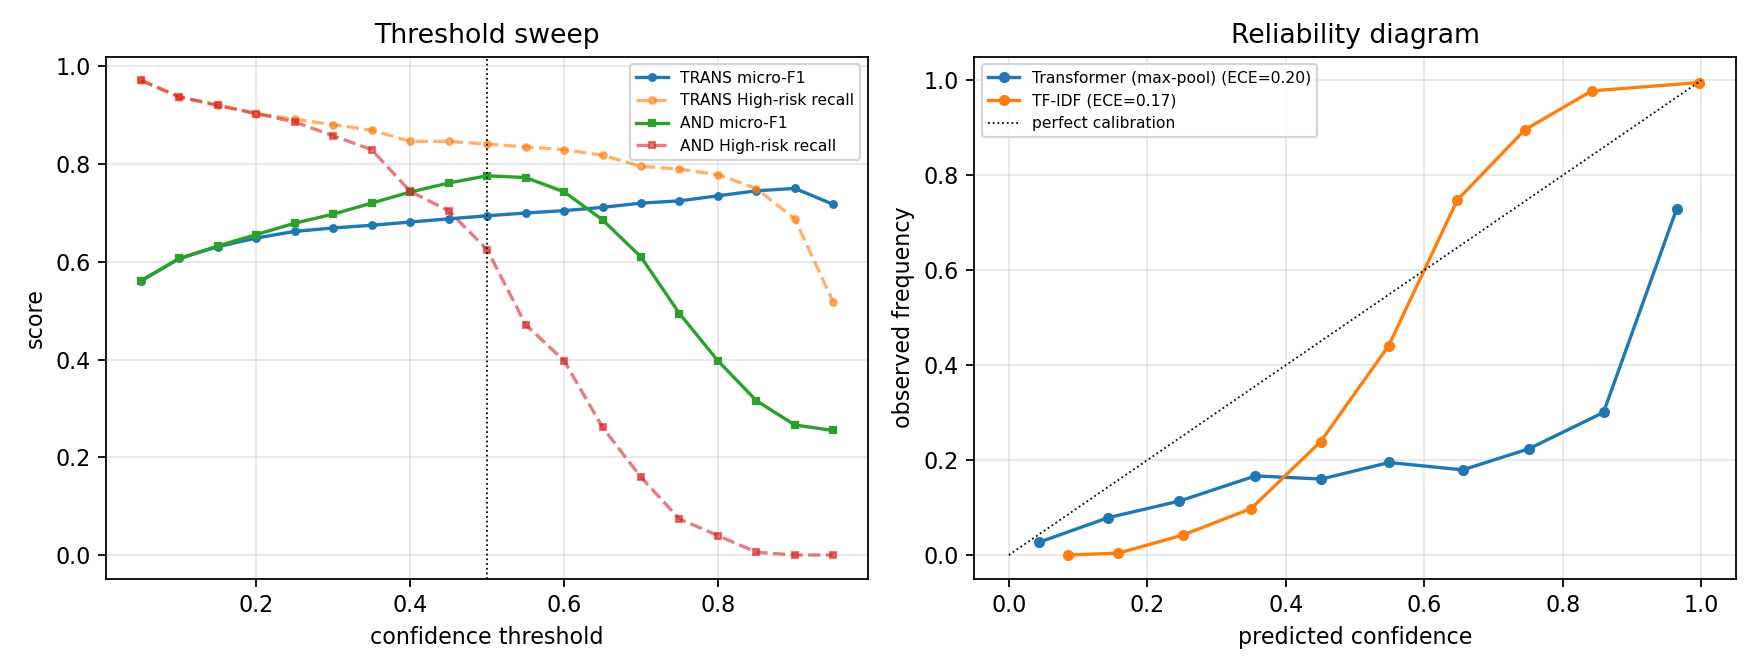
\includegraphics[width=\columnwidth]{threshold_calibration.png}
\caption{Threshold sweep (left) and reliability diagram (right).}
\label{fig:cal}
\end{figure}

\subsection{Span Extraction}
Given an answer-bearing window, token-F1 is 0.763 (contract-clustered 95\% CI
$[0.740,0.782]$), with 82.7\% of predictions overlapping the gold span at F1 $\geq 0.5$. The
clustered interval is roughly twice the width obtained by resampling clauses independently,
which is the practical cost of ignoring within-contract correlation.

\subsection{Summarization}
\label{sec:summ}
CUAD contains no plain-English rewrites, so the 41 targets were author-written; every test
clause is scored against one of only 41 unique strings. To separate template reproduction from
summarization we scored the same 150 held-out clauses against a second, clause-specific
reference set drafted independently of the model (Table~\ref{tab:summ}).

\begin{table}[!t]
\caption{ROUGE-L under two reference sets, same 150 clauses}
\label{tab:summ}
\centering
\begin{tabular}{llc}
\toprule
\textbf{System} & \textbf{References} & \textbf{ROUGE-L}\\
\midrule
Fine-tuned FLAN-T5 & 41 templates       & 0.775\\
Fine-tuned FLAN-T5 & clause-specific    & 0.116\\
Zero-shot FLAN-T5  & clause-specific    & 0.299\\
\emph{Template alone, no model} & clause-specific & 0.115\\
\bottomrule
\end{tabular}
\end{table}

The fine-tuned model emits one of the 41 templates \emph{verbatim on 100\% of inputs} --- the
correct one 70\% of the time. A constant lookup table matches its score. The task became
41-way classification, and the metric did not register the change. Notably, a template-emitting
model cannot hallucinate in the usual sense; it fails instead by producing fluent, confident
text about a different provision, which is undetectable from the output alone.

\subsection{Qualitative Error Analysis}
Inspecting the highest-confidence mistakes identifies three recurring patterns. \emph{Lexical
triggers without the obligation:} a royalty clause deducting ``insurance costs'' is flagged as an
\emph{Insurance} covenant by both models (0.82/0.97) --- the vocabulary is present, the obligation
is not. \emph{Concept without vocabulary:} a term requiring ``a cancellation fee of \$5{,}000 per
month multiplied by the number of months remaining'' is textbook liquidated damages and is missed by
both models (0.21/0.02), because the category's vocabulary never appears and 24 positive training
contracts are too few to learn the concept. \emph{Annotation disagreement:} some rare-category
``failures'' are cases where the gold label is itself arguable, so the 0.000 scores on the rare tail
mix model error with label ceiling effects. On the span side, failures include degenerate
single-token predictions and confident answers drawn from windows that cannot contain the clause ---
both symptoms of an extractor with no way to abstain.

\subsection{End-to-End Evaluation}
\label{sec:e2e}
Running all stages in series over the 1{,}348 gold clauses in the test contracts gives
Table~\ref{tab:e2e}. A clause survives only if its category is detected, the span extracted
from the \emph{selected} window overlaps the gold clause at token-F1 $\geq 0.5$, and the risk
label is correct.

\begin{table}[!t]
\caption{End-to-end attrition over 1{,}348 gold clauses}
\label{tab:e2e}
\centering
\begin{tabular}{lcc}
\toprule
\textbf{Stage} & \textbf{Surviving} & \textbf{Share}\\
\midrule
Gold clauses            & 1{,}348 & 100.0\%\\
Presence detected       & 1{,}052 & 78.0\%\\
Span overlap $\geq 0.5$ & 293     & \textbf{21.7\%}\\
Risk label correct      & 293     & 21.7\%\\
\bottomrule
\end{tabular}
\end{table}

Multiplying the component figures predicts $\approx$64\%; the pipeline delivers a third of
that. Decomposing the loss over the 1{,}052 detected clauses: the selected window contains the
gold text only 68.3\% of the time, and even then extraction succeeds 39.7\% of the time against
82.7\% in isolation. The first cause is a detector reused as a locator --- max-pooling was
trained to answer whether a window contains a clause, not which window does. The second is the
re-centring used at training time: legitimate with respect to leakage, but it narrows the
distribution the model can read, and mean token-F1 falls from 0.763 to 0.386. Both are
addressable without additional parameters.

\section{Deployment Observations}
The pipeline is deployed as a local web application. Three measurements bear on whether such a
system should be trusted by a non-specialist. \textbf{Latency:} a median-length contract takes
27.1\,s and the worst case 32.4\,s on CPU, with models resident. \textbf{Truncation:} a
30-window cap bounds latency but reads only the first 45{,}500 characters, and 38.4\% of CUAD
contracts exceed that --- clauses beyond the cap cannot be detected, a limitation invisible in
any of the offline metrics reported above. \textbf{Calibration:} the score presented to the user
as confidence has ECE 0.201 and Brier score 0.194, so the displayed value should not be read as
a probability of correctness.

Combined with the end-to-end result, this suggests a specific interface discipline: the category
label and its risk badge are considerably more reliable than the quoted clause text beneath
them, and an interface of this kind should present extracted spans as pointers to a location
rather than as authoritative quotations.

\section{Threats to Validity}
\label{sec:threats}
\textbf{Internal.} No hyperparameter was tuned, which protects the held-out evaluation but
leaves the transformer untuned against a baseline with little to tune; the threshold control
quantifies part of this.
\textbf{Construct.} ROUGE-L measures its reference set rather than the task, as
Section~\ref{sec:summ} demonstrates directly; micro-F1 does not measure user harm, as
Section~\ref{sec:risk} demonstrates. The risk bands are our own construct and have not been
validated by anyone with legal training, so Table~\ref{tab:risk} inherits that limitation.
\textbf{External.} All results come from 510 US commercial contracts drawn from SEC filings, in
English. No contract outside that corpus has been evaluated.
\textbf{Statistical.} Three variance sources were measured and all exceed the ensemble margin;
three seeds is a small sample for a standard deviation; per-category statistics on the rare tail
are not meaningful individually.

\section{Discussion}
The results support a general recommendation with three parts. First, a margin should be compared
against its own noise before it is reported, and the relevant noise has at least three components ---
test-set resampling, training stochasticity, and the draw of the split itself --- of which the last is
both the largest here and the most frequently omitted. Second, an evaluation should be run on the
assembled system, because stage-wise scores compose optimistically: ours over-predict by a factor of
three, and the discrepancy localizes to interfaces between components rather than to any component.
Third, the reported metric should be checked against the objective the system exists to serve; where
these diverge, as in Section~\ref{sec:risk}, optimizing the metric actively degrades the system's
usefulness.

None of these checks required additional compute or data. Each required asking a question that the
component-wise reporting convention does not prompt.

\section{Conclusion}
On a strict held-out protocol, a full-document lexical baseline beats a windowed transformer at
clause presence classification, and the result survives controls for training budget, random
seed, aggregation rule and decision threshold. More consequentially, the assembled pipeline
retains 21.7\% of gold clauses where its component scores predict $\approx$64\%, and the
configuration that maximizes aggregate micro-F1 is the worst available choice for the clauses
carrying the highest risk. We suggest that pipeline-level survival and a purpose-weighted
metric belong alongside component scores in any system of this kind, and that a margin should
be compared against seed and split variance --- not only against a bootstrap interval --- before
being reported as a result.

Future work: obtaining expert validation of the risk taxonomy; a purpose-weighted selection
protocol on a validation split; calibration of the confidence estimate; abstention for the span
model; and faithfulness-aware evaluation of generated explanations.

\section*{Acknowledgment}
The authors thank Utsha Kumar Roy for insisting on a strict held-out evaluation protocol, which
shaped how honestly this work reports its results.

\begin{thebibliography}{99}
\bibitem{cuad} D. Hendrycks, C. Burns, A. Chen, and S. Ball, ``CUAD: An expert-annotated NLP dataset for legal contract review,'' in \emph{Proc. NeurIPS Datasets and Benchmarks}, 2021.
\bibitem{squad} P. Rajpurkar, J. Zhang, K. Lopyrev, and P. Liang, ``SQuAD: 100,000+ questions for machine comprehension of text,'' in \emph{Proc. EMNLP}, 2016, pp. 2383--2392.
\bibitem{legalbert} I. Chalkidis \emph{et al.}, ``LEGAL-BERT: The muppets straight out of law school,'' in \emph{Findings of EMNLP}, 2020, pp. 2898--2904.
\bibitem{lexglue} I. Chalkidis \emph{et al.}, ``LexGLUE: A benchmark dataset for legal language understanding in English,'' in \emph{Proc. ACL}, 2022.
\bibitem{longformer} I. Beltagy, M. E. Peters, and A. Cohan, ``Longformer: The long-document transformer,'' \emph{arXiv:2004.05150}, 2020.
\bibitem{mil} O. Maron and T. Lozano-P\'erez, ``A framework for multiple-instance learning,'' in \emph{Proc. NIPS}, 1998, pp. 570--576.
\bibitem{t5} C. Raffel \emph{et al.}, ``Exploring the limits of transfer learning with a unified text-to-text transformer,'' \emph{JMLR}, vol. 21, no. 140, pp. 1--67, 2020.
\bibitem{flan} H. W. Chung \emph{et al.}, ``Scaling instruction-finetuned language models,'' \emph{JMLR}, vol. 25, no. 70, pp. 1--53, 2024.
\bibitem{manor} L. Manor and J. J. Li, ``Plain English summarization of contracts,'' in \emph{Proc. Natural Legal Language Processing Workshop}, 2019, pp. 1--11.
\bibitem{maynez} J. Maynez, S. Narayan, B. Bohnet, and R. McDonald, ``On faithfulness and factuality in abstractive summarization,'' in \emph{Proc. ACL}, 2020, pp. 1906--1919.
\bibitem{factcc} W. Kry\'sci\'nski, B. McCann, C. Xiong, and R. Socher, ``Evaluating the factual consistency of abstractive text summarization,'' in \emph{Proc. EMNLP}, 2020, pp. 9332--9346.
\bibitem{rouge} C.-Y. Lin, ``ROUGE: A package for automatic evaluation of summaries,'' in \emph{Text Summarization Branches Out}, 2004, pp. 74--81.
\bibitem{bertscore} T. Zhang, V. Kishore, F. Wu, K. Q. Weinberger, and Y. Artzi, ``BERTScore: Evaluating text generation with BERT,'' in \emph{Proc. ICLR}, 2020.
\bibitem{calibration} C. Guo, G. Pleiss, Y. Sun, and K. Q. Weinberger, ``On calibration of modern neural networks,'' in \emph{Proc. ICML}, 2017, pp. 1321--1330.
\bibitem{distilbert} V. Sanh, L. Debut, J. Chaumond, and T. Wolf, ``DistilBERT, a distilled version of BERT,'' in \emph{Proc. EMC$^2$ Workshop, NeurIPS}, 2019.
\end{thebibliography}

\end{document}
